\documentclass[a4paper,12pt]{report}
\usepackage[T2A]{fontenc}
\usepackage[utf8]{inputenc}
\usepackage[english,russian]{babel}
\usepackage{graphicx}
\usepackage{wrapfig}
\usepackage{mathtext} 				% русские буквы в фомулах
\usepackage{amsmath,amsfonts,amssymb,amsthm,mathtools} % AMS
\usepackage{icomma} % "Умная" запятая: $0,2$ --- число, $0, 2$ --- перечисление
\usepackage{capt-of}
\usepackage{appendix}
\usepackage{multirow}
\usepackage{hyperref}
\usepackage{floatrow}
\usepackage[left=2cm,right=2cm,
    top=2cm,bottom=2cm,bindingoffset=0cm]{geometry}
\usepackage{multicol} % Несколько колонок
\usepackage{gensymb}
\title{Отчёт по лабораторной работе №12

Определение петли гистерезиса
ферромагнетика магнитооптическим методом}
\author{Плюскова Н.А. Б04-004 }
\date{\today}

\begin{document}

\maketitle


\section*{1. Теоретические данные}
 Принято различать следующие типы веществ в зависимости от их магнитных свойств:
\begin{itemize}
    \item парамагнетики - вещества во слабыми магнитными свойствами, в отсутствие внешнего магнитного поля магнитный момент равен нулю. В парамагнетиках отдельные атомы имеют собственный магнитный момент, внешнее магнитное поле частично упорядочивает направления этих магнитных моментов. Магнитная восприимчивость парамагнетиков положительна.
    \item диамагнетики - также вещества со слабыми магнитными свойствами. Собственный магнитный момент атомов равен нулю, индуцированный магнитный момент в соответствии с правилом Ленца направлен против магнитного поля. Магнитная восприимчивость диамагнетиков отрицательна.
    \item ферромагнетики - существует спонтанная намагниченность вещества, обусловленная внутренними взаимодействиями, приводящими к параллельной ориентации магнитных моментов отдельных атомов.
\end{itemize}

Связь величины вектора магнитной индукции в веществе ($B$), намагниченности вещества ($I$) и напряжённости внешнего магнитного поля ($H$):
\begin{equation}
    B = H + 4\pi I
\end{equation}
Связь магнитной проницаемости $\mu$ с магнитной восприимчивостью $\chi$:
\begin{equation}
    \mu = 1 + 4\pi \chi
\end{equation}

Теории, построенные для выяснения природы взаимодействий, приводящих к появлению спонтанной намагниченности, учитывают не только молекулярные, но и обменные взаимодействия. Обменное взаимодействие зависит от ориентации спинов электронов в кристалле (электронов За и 4Е оболочек соседних атомов). Также обменное взаимодействие может переноситься диамагнитными ионами или электронами проводимости.

Для описания магнитной структуры ферромагнетиков и антиферромагнетиков (а также некоторых других веществ) используют понятие домена. Вейсс предположил, что магнитные образцы состоят из множества малых областей, называемых доменами, в каждой из которых намагниченность равна намагниченности насыщения, но направления векторов намагниченности не обязательно должны быть параллельными друг другу. Доменная структура образуется в магнетике за счёт более слабых энергетических взаимодействий по сравнению с обменными (энергии размагничивания, анизотропии, зеемановской энергии). Доменная граница представляет собой область, в которой происходит плавный разворот вектора намагниченности от направления в одном домене к направлению в соседнем домене.

При отсутствии внешнего магнитного поля результирующий магнитный момент ферромагнетика равен нулю. Если состояние, при котором намагниченность и внешнее магнитное поле, считать начальным, то зависимость $B(H)$ для ферромагнетика имеет вид, изображённый на, рис. \ref{I}.

\begin{figure}[H]
    \centering
    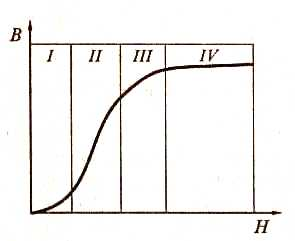
\includegraphics[width=0.4\linewidth]{pic1.png}
    \caption{Кривая намагничивания вещества} \label{I}
\end{figure}

1. Область начального обратимого намагничивания. Изменение намагниченности обусловлено обратимыми процессами, связанными с упругим смещением доменных границ

2. Область, соответствующая необратимому смещению доменных границ

3. Область приближения к насыщению. Направление вектора намагниченности отдельных областей приближается к направлению внешнего поля

4. Область парапроцесса. Наблюдается слабый рост намагниченности

$\textbf{Гистерезис}$ - это явление, состоящее в том, что для одних и тех же значений напряжённости внешнего магнитного поля получаются разные значения намагниченности (при уменьшении магнитного поля после получения основной кривой значения намагниченности не совпадают с последней). Гистерезис обусловлен стремлением ферромагнитного материала препятствовать изменению своего состояния при внешнем воздействии. Типичная петля гистерезиса ферромагнетика представлена на рис. \ref{hysteresis} $\textbf{Коэрцитивная сила}$ $H_{c}$ - значение магнитного поля, при котором намагниченность станет равной нулю. Поле насыщения $H_{max}$ (или $H_{s}$) - значение магнитного поля, при котором достигается максимальная намагниченность образца.

\begin{figure}[H]
    \centering
    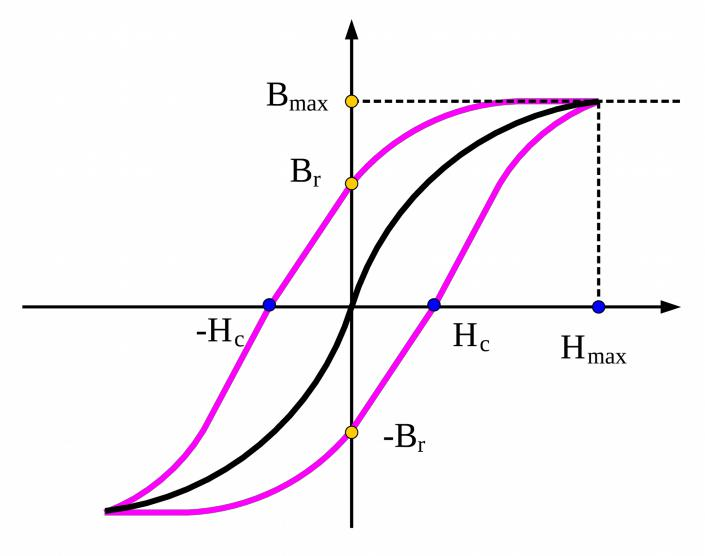
\includegraphics[width=0.4\linewidth]{pic2.png}
    \caption{Петля гистерезиса} \label{hysteresis}
\end{figure}

\section*{2. Экспериментальная установка}
Измерение петли гистерезиса проводится магнитооптическим методом с использованием эффекта Фарадея, который заключается во вращении плоскости поляризации линейно поляризованного света при прохождении намагниченного вещества.

\begin{figure}[H]
    \centering
    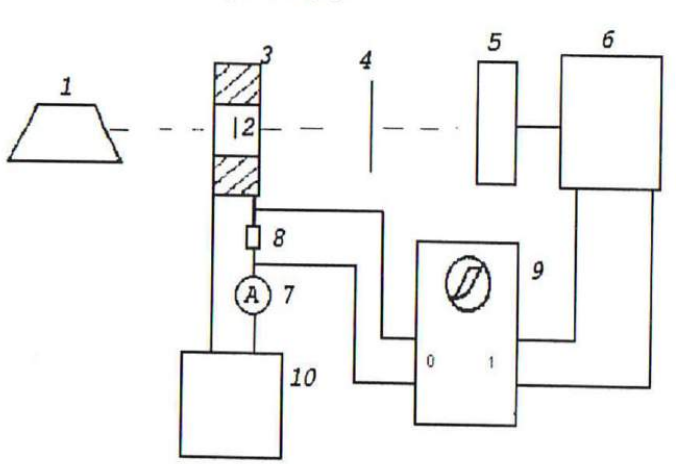
\includegraphics[width=0.4\linewidth]{pic3.png} \label{setup}
    \caption{Блок-схема установки: 1 - лазер, 2 - образец, 3 - катушка, 4 — анализатор, 5 — фотоприёмник, 6 - усилитель,
7 — амперметр, 8 — резистор, 9 — виртуальный осциллограф, 10 — генератор переменного напряжения}
\end{figure}

Лазер излучает линейно поляризованный свет, который проходит через образец с намагниченностью $I$, плоскость поляризации поворачивается на некоторый угол $\psi$, пропорциональный проекции намагниченности на вектор распространения света. Затем луч идет через анализатор, который представляет собой поляроид. Интенсивность выходного сигнала изменяется в
соответствии с законом Малюса: $I = I_{0}cos^2\theta$, где $\theta$ — угол между плоскостью поляризации входного излучения и разрешенным направлением поляроида. Далее луч света обрабатывается фотоприёмником, выходной сигнал подается на канал 1.

\section*{3. Результаты эксперимента и обработка данных}
Соберём установку, согласно блок-схеме (рис. \ref{setup}). Включим лазер, усилитель, источник питания; анализатор установим в положение 45° (амплитуда сигнала в таком случае будет максимальной).

Определим оптимальное значение резистора. Ток в катушке равен 1.85 А, напряжение 25 В. С учётом того, что ток в установке переменный, сопротивление будет равно
 \begin{equation*}
     R = \frac{V}{\sqrt{2} I} = 9.55 \text{ Ом}
 \end{equation*}

Подключим входные сигналы к цифровому осциллографу. Получим на экране зависимости напряжения на каналах 0 и 1 от времени.

Используя полученные данные, построим петлю гистерезиса $B(H)$ исследуемого образца. Построим зависимость величины выходного напряжения с усилителя от величины магнитного поля. Величина напряжения $U$ на канале 0 будет связана с напряжённостью магнитного поля $H$ по следующей формуле:

  \begin{equation*}
     H =  \alpha \frac{U}{R}
 \end{equation*}
где $\alpha$ =150 Э/А - калибровочный коэффициент катушки, $R$ = 9.55$\Omega$ - оптимальное значение резистора. Напряжение на канале 1 пропорционально проекции намагниченности образца на направление
распространения света. Отнормируем показания с канала 1 по максимальному значению, получим значения, пропорциональные намагниченности образца в процентах. Полученный график представлен на рис. 4.

\begin{figure}[H]
    \centering
    \includegraphics[width=0.8\linewidth]{pic4.png} \label{exp}
    \caption{Петля гистерезиса исследуемого образца}
\end{figure}

По графику определим магнитные параметры исследуемого образца: коэрцитивную силу $H_{c}$ (полуширина петли на уровне $B$ = 0 $\%$) и поле насыщения $H_{s}$ (значение $H$ при $B$ = 100 $\%$)
 
 \begin{equation*}
     H_{c} = 6.25 \text{ Э}
 \end{equation*}
 \begin{equation*}
     H_{s} = 8 \text{ Э}
 \end{equation*}
 
\section*{4. Вывод}
При выполнении данной работы мы ознакомились с принципами применения магнитооптических методов для исследования прозрачных магнетиков, а также, получив кривую гистерезиса для ферромагнитного образца, удалось найти некоторые его параметры, а именно коэрцитивную силу $H_{c} = 6.25$ Э, и поле насыщения $H_{s} = 8$ Э. Также на примере исследования магнитных свойств магнетиков мы изучили основы и принципы применения вычислительной техники для организации автоматизированного сбора и анализа экспериментальных данных физического прибора.

\end{document}
